\documentclass[10pt,a4paper,twoside]{article}
\usepackage[utf8]{inputenc}
\usepackage{amsmath}
\usepackage{amsfonts}
\usepackage{amssymb}
\usepackage{graphicx}

%Note: Jeg har sat den op til at være 2-sidet, hvilket giver skiftende margener
%      Det ser lidt underligt ud i PDF'en, men jeg tror det giver en god effekt


\begin{document}
\title{Enhancements for Monte Carlo Tree Search in The Mario AI Framework}
\date{May 22, 2013}
\author{\\Emil Juul Jacobsen\\\texttt{ejuu@itu.dk}        
        \and \\Rasmus Greve\\\texttt{ragr@itu.dk}
        \and \emph{Supervisor:}\\Julian Togelius\\\texttt{juto@itu.dk}}
\maketitle

\begin{center}
IT University of Copenhagen
\end{center}

\begin{abstract}
(Bare copy/paste-ish fra projektbasen, skal skrives om!)
In this experiment we explore different implementations and enhancements of the Monte Carlo Tree Search algorithm for an AI, in order to evaluate their performance and results in the Super Mario AI Benchmark tool. 
We have implemented the basic MCTS algorithm in the Mario AI 
Framework and characterised the performance and identification of 
the strengths and weaknesses of the algorithm relative to the 
framework. We have identified a set of refinements and alterations of the algorithm 
and through implementation and evaluation of these individually we came up
with compositions that greatly increase the performance of the AI.
\end{abstract}

\pagebreak

\section{Introduction}
In this experiment we explore different implementations and enhancements of the Monte Carlo Tree Search algorithm for an AI, in order to evaluate their performance and results in the Super Mario AI Benchmark tool. 

\section{Background}
\begin{itemize}
\item Om MCTS \cite{mctssurvey}
\item Om UCB og UCT \cite{mctssurvey} måske også \cite{mspacman}
\item (kort!) Om The Mario AI Framework  \cite{mario}
\end{itemize}



\section{Approach and Improvements}

\subsection{Monte Carlo Tree Search with UCT}
\cite{mctssurvey}
\subsection{Softmax Backup}
\subsection{High domain knowledge}
\subsubsection{Limited actions}
\subsubsection{Hole detection}
\subsection{Macro actions}
\cite{salesman}
\subsection{Heuristic Partial Tree Expansion Policy}
\subsection{Checkpoints}

\subsection{(Combination)}

\section{Results}
Her er noget tekst

\begin{figure}[h] %h: ca her, t: sidetop, b: sidebund
\centering
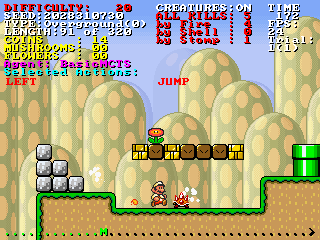
\includegraphics[width=6cm]{img/Forfulgt}
\caption{Mario being followed}
\label{fig:followed}
\end{figure}

Her er noget mere tekst, som det ses på billede \ref{fig:followed}

\section{Conclusion}

\section{Some Sums DEMO}

Here are a few sums\footnote{Additions of sets of numbers}  I know.\label{sec:formulas}

\begin{eqnarray}
1+2+3+\cdots+n&=&\frac{n(n+1)}{2}\label{linear}\\
1^2+2^2+3^2+\cdots+n^2&=& \frac{n(n+1)(2n+1)}{6}\label{squares}\\
1^3+2^3+3^3+\cdots+n^3&=& \frac{n^2(n+1)^2}{4}\label{cubes}
\end{eqnarray}

I can find the sum of the first 10 squares easily with formula~(\ref{squares}) above.

\pagebreak

\section{A Cool Relationship DEMO}

Take a look at formulas~(\ref{linear}) and~(\ref{cubes}) on
page~\pageref{linear} of section~\ref{sec:formulas}. Notice that the
right side of~(\ref{cubes}) is the square of the right side
of~(\ref{linear}).


\begin{thebibliography}{99}

\bibitem{mctssurvey}
  C. B. Browne, E. Powley, D. Whitehouse, S. M. Lucas, P. I. Cowling, P. Rohlfshagen, S. Tavener, D. Perez, S. Samothrakis, and S. Colton, “A survey of monte carlo tree search methods,” Computational Intelligence and AI in Games, IEEE Transactions on, vol. 4, no. 1, pp. 1–43, 2012.

\bibitem{civii}
S. R. K. Branavan, D. Silver, and R. Barzilay, “Non-linear monte-carlo search in civilization ii,” in Proceedings of the Twenty-Second international joint conference on Artificial Intelligence-Volume Volume Three, 2011, pp. 2404–2410.

\bibitem{salesman}
E. J. Powley, D. Whitehouse, and P. I. Cowling, “Monte Carlo Tree Search with macro-actions and heuristic route planning for the Physical Travelling Salesman Problem,” in Computational Intelligence and Games (CIG), 2012 IEEE Conference on, 2012, pp. 234–241.

\bibitem{mspacman}
T. Pepels and M. H. Winands, “Enhancements for Monte-Carlo Tree Search in Ms Pac-Man,” in Computational Intelligence and Games (CIG), 2012 IEEE Conference on, 2012, pp. 265–272.

\bibitem{mario}
S. Karakovskiy and J. Togelius, “The mario ai benchmark and competitions,” Computational Intelligence and AI in Games, IEEE Transactions on, vol. 4, no. 1, pp. 55–67, 2012.

\end{thebibliography}

\end{document}